\documentclass[12pt]{article}
\usepackage[letterpaper]{geometry}
\usepackage{hyperref}
\usepackage{textcomp}
\usepackage{listings}
\usepackage{graphicx}
\usepackage{tabularx}
\usepackage{color}
\definecolor{darkred}{rgb}{0.5,0,0}
\definecolor{darkblue}{rgb}{0,0,0.5}
\definecolor{darkgreen}{rgb}{0,0.5,0}
\lstset{
   captionpos=b,
   basicstyle=\ttfamily,
   frame=lines,
   tabsize=4,
   showstringspaces=false,
   commentstyle=\color{darkgreen},
   keywordstyle=\color{darkblue},
   stringstyle=\color{darkred},
   identifierstyle=\bfseries, 
   escapechar={\%}
}


\title{CS 130 LONI 2: Pipeline Converter Design Document}
\author{S. Achour, K. C. Ho, R. Soberano, C. Tandiono,\\ N. Van Hoogenstyn, J. Yoon}
\begin{document}
\maketitle
\pagebreak
\label{toc}
\phantomsection\pdfbookmark[1]{Contents}{contents}
\tableofcontents
\pagebreak
\section{Introduction}
\subsection{Purpose}
This software design document describes the architecture and system design of the Laboratory of Neuro Imaging (LONI) Pipeline Converter. It provides a general overview of its structure, interface, and functionality. This intended audiences for this document are LONI stakeholders, the project developers, and the testers.

\subsection{Scope}

The Pipeline Converter is for researchers in the life sciences that wish to share their work and utilize the work of others in the form of workflows made in the LONI Pipeline, Taverna, or Galaxy workflow editors. The goal of the project is to provide a simple way for researchers working with different workflow editors to examine and reenact each other's experiments. It allows the researchers to access all the possible experiments in LONI, Taverna, and Galaxy.

\subsection{Overview}

The overall organization of the document's contents are laid out in the Contents on page~\pageref{toc}.

\subsection{Reference Material}
\begin{itemize}
\item GSON reference: \url{http://code.google.com/p/google-gson/}
\item XStream reference: \url{http://xstream.codehaus.org/}
\item Pipeline documentation: \url{http://pipeline.loni.ucla.edu/support/xml-overview/}
\item Taverna documentation: \url{http://taverna.googlecode.com/svn/taverna/dev/xsd/trunk/t2flow/}
\item Galaxy documentation: \url{http://wiki.g2.bx.psu.edu/Admin/Tools/Tool\%20Config\%20Syntax}
\end{itemize}

\subsection{Definitions and Acronyms}
\begin{itemize}
\item \textbf{LONI}--Laboratory of Neuro Imaging
\item \textbf{OTS}--object tree structure (explained further in section~\ref{ots})
\item \textbf{Converter}--the Pipeline Converter software whose design is described in this document
\end{itemize}

\section{System Overview}

The Pipeline Converter's main function will be to convert workflow files between the LONI Pipeline, Taverna, and Galaxy workflow editors. Specifically, the Converter will provide the following functions:

\begin{itemize}
\item    Convert a LONI Pipeline (\texttt{.pipe} file) workflow to an equivalent Taverna (\texttt{.t2flow} file) workflow
\item     Convert a LONI Pipeline (\texttt{.pipe} file) workflow to an equivalent Galaxy (\texttt{.ga} file) workflow
\item    Convert a Taverna (\texttt{.t2flow} file) workflow to an equivalent LONI Pipeline (\texttt{.pipe} file) workflow
\item    Convert a Galaxy (\texttt{.ga} file) workflow to an equivalent LONI Pipeline (\texttt{.pipe} file) workflow
\end{itemize}

The Pipeline Converter will be a platform-independent Java utility. It will be comprised of three major subsystems: a parser, a converter, and a generator. Each of these will be explained in more detail in section~\ref{archdesign}.

\section{System Architecture}

\subsection{Architectural Design}
\label{archdesign}

The system architecture will be implemented as detailed in figure~\ref{fig:architecture}. The overall program consists of three main subsystems: the parser, the converter, and the generator. 

\begin{figure}[htbp]
\centering
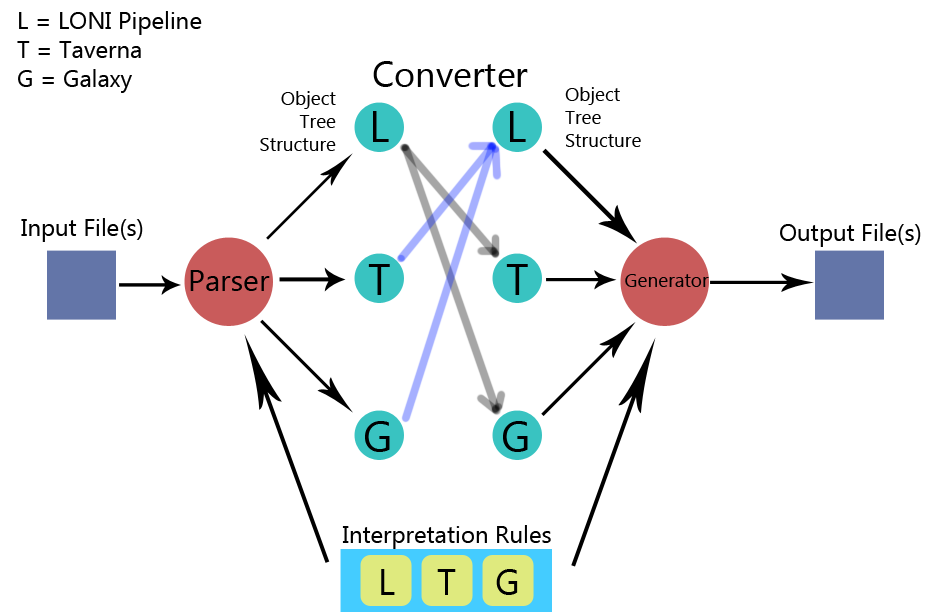
\includegraphics[width=\textwidth]{architecture.png}
\caption{System architecture overview.}
\label{fig:architecture}
\end{figure}

\subsubsection{Parser}
\label{ots}

Each file format has its own Object Tree Structure (OTS). Each OTS is comprised of objects from a set of classes unique to the corresponding file format. The OTS's implemented in this project have a 1-to-1 mapping to the tags and elements in the file format. The OTS for input files is created by the Parser.

The parser reads in a input file and generates the Object Tree Structure for that file using rules specific to the format. Note the parser extracts information from a standard data arrangement format (such as XML), while the Object Tree Structure and rules are defined by the format of the data itself. This includes all the elements and tags that the format uses, and the hierarchy and order in which they are arranged. The parser is able to correctly interpret the input file once the structure-matching rules have been defined. Structure matching rules define relationships between portions of the input file and objects that make up the OTS. These rules are specific to the file format, and are defined in the specification object. Third party XStream library is used to make the parser. This library requires only one set of constraints to parse and generate files, and support both operations.  

As an example, consider the simple portion of hierarchical XML code in listing~\ref{xml-sample}.


\noindent
\lstset{language=HTML}
\begin{lstlisting}[frame=single,label=xml-sample,caption=A sample piece of hierarchical XML code.]
<modulegroup name="the_group">
	<module><!-- ... more XML ... --></module>
	<module><!-- ... more XML ... --></module>
	<module><!-- ... more XML ... --></module>
</modulegroup>
\end{lstlisting}

This portion of the XML tree can mapped to the ModuleGroup name, as seen in listing~\ref{java-sample}. The enclosing modules are mapped to a Module List and the name is mapped to the ``name'' field.

\noindent
\lstset{language=Java}
\begin{lstlisting}[frame=single,label=java-sample,caption=Sample class definition for ModuleGroup.]
class ModuleGroup {
	String name;
	List<Module> moduleList;
}
\end{lstlisting}

The rules for this mapping may be something along the lines of that in listing~\ref{map-sample}.
\noindent
\\
\begin{lstlisting}[frame=single,label=map-sample,caption=Sample mapping from XML to Java.]
map("modulegroup", /* ModuleGroup class */);
map("module", /* Module class */);
map("modulegroup/name", /* name in ModuleGroup class */);
\end{lstlisting}

After parsing is done, the resulting OTS can then be handed off to the converter, the next major subsystem of the program.

\subsubsection{Converter}

The converter's role is to translate the OTS of the input file format into an equivalent OTS of the output file format. It knows what workflow elements map to other workflow elements between LONI Pipeline, Taverna, and Galaxy. The converter acts on the OTS that is passed in from the parser. The converter will visit all nodes in the input OTS recursively and build the output OTS from the bottom up by converting each node it visits. Once the converter performs its job, the resulting OTS is given to the generator.


\subsubsection{Generator}

The generator is the last major subsystem of the program. It takes the output OTS as input and generates the output file. This step generates the converted files from the output OTS. The output file will be functionally analagous the input file, but will work with a different workflow editor depending on the output format specified by the user. Like the parser, the generator is created with a set of rules by the specification object. Since parsing and generating are symmetric operations, these rules are essentially the same for both the parser and the generator. Third party GSON library is used to make the generator. This library require only one set of constraints to parse and generate files, and support both operations.  

\subsection{Decomposition Description}

\subsubsection{Parsers and Generators}



\paragraph{Description}

The inheritance digram for our parsers and generators can be seen in figure~\ref{fig:inheritance}. Parsers are responsible for parsing a file into an object tree structure, and Generators are responsible for converting an object tree structure to a file. Both can be configured to output various output tree structures based on a set of rules. The Specification classes configure the Parsers and Generators for the particular format specification. For example, the GalaxySpecification Specification class configures the Parser to parse to a Galaxy Workflow tree, and the Generator to output a file from a Galaxy Workflow tree.

\begin{figure}[htbp]
\centering
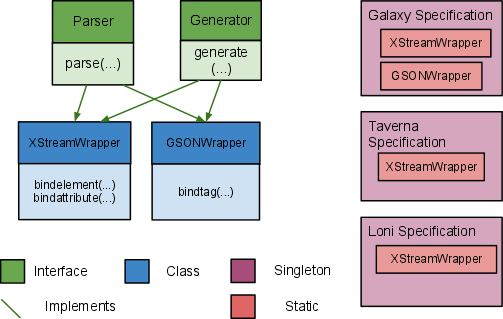
\includegraphics[width=\textwidth]{inheritance.png}
\caption{Inheritance diagram: is-a and has-a relationships, singleton/static fields.}
\label{fig:inheritance}
\end{figure}

In this design, we use two open-source parsing components, XStream and GSON. Both parsers reflectively map the parsed file a specified object using a set of bindings outlined by the user. To avoid directly using the third-party libraries, we use wrapper classes to indirectly access the subset of functions needed for each parser. The wrappers hide the complexities of setting up the third party generators and only expose a fraction of their features. These  two wrappers implement both of the the parser and generator classes.The parser interface enforces the implementation of file parsing and string parsing methods, and the generator enforces that object to string and object to file generation functions are implemented. With these interfaces implemented, wrappers can be used interchangeably as Parsers and Generators. 



\paragraph{Interaction}


The specification classes hold some subset of wrapper object, as seen in figure~\ref{fig:interaction}. The specification binds rules to the enclosed wrappers according to the format of the workflow file. The rule binding functions are different for each wrapper.  Other classes can use these wrappers through the Specification's getter methods, which return either a parser or a generator for each file type. This way, the specification can customize the parser without directly modifying the third-party program using the interface provided by the wrapper. The wrapper interface is not visible to classes asking for the parser or a generator for a file format, since a Parser or a Generator object is returned. Note there is no common wrapper interface. Since there is a great deal of variation between third party parsing libraries, the binding functions available would vary greatly from wrapper to wrapper. Using a wrapper interface may be too restrictive for parsers that may be added in the future.

\begin{figure}
\centering
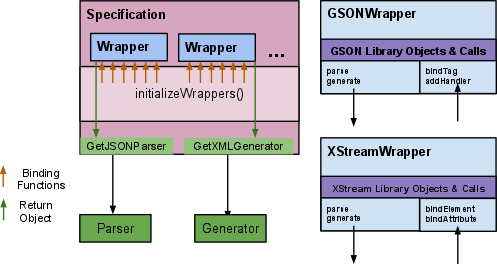
\includegraphics[width=\textwidth]{interaction.png}
\caption{Interaction diagram: wrappers, specification, external Classes.}
\label{fig:interaction}
\end{figure}

\subsubsection{Converter}

The converter (seen in figure~\ref{fig:conversion}) takes an OTS for one file format and changes it to another file format. Each conversion permutation has a corresponding visitor class that accepts a source OTS and outputs the desired OTS. A visitor is a type of class that starts at the root node of the OTS, and recursively visits all the subnodes in some order. In a visitor, each type of node has a visit function. If the node is polymorphic, the most specific visit function is ascertained using double-dispatch or dynamic type checking.  A conversion visitor is a type of visitor. In a conversion visitor, each visit function processes a node type from the source OTS and converts it into a node from the destination OTS. This destination OTS node is returned.  The end result is a tree visitor that recursively builds up the destination tree from the source tree.

\begin{figure}[htbp]
\centering
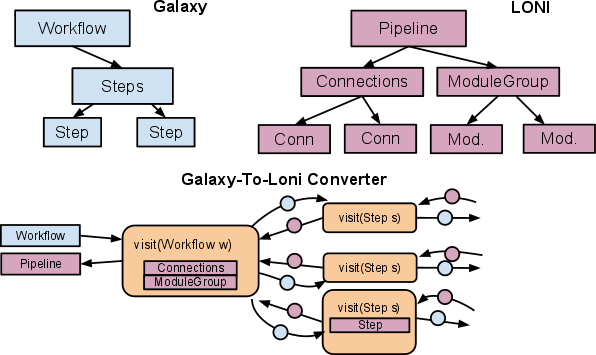
\includegraphics[width=\textwidth]{conversion.png}
\caption{Diagram of recursive conversion from Galaxy OTS to LONI OTS. Objects listed inside visit boxes are constructed in that visit call.}
\label{fig:conversion}
\end{figure}

The Galaxy visitor in particular will require a Toolbox object in addition to the workflow. the toolbox maps all the tool ids to tool paths. Tool specifications request tool objects from the Toolbox object, which parses and caches tools when necessary.

\paragraph{Visitor}

For the converter, we are applying the visitor design pattern. A different visitor interface is required to be implemented for each OTS, as shown in figure~\ref{fig:visitorinheritance}.  The visitor interface contains visit functions for all the objects that are part of the format's OTS. A Converter is required to implement the interface if the source OTS visitor to ensure none of the object types are skipped and avoid undefined behaviour. The most specific visit function in the visitor is called for a derived object in the OTS.  If a subset of visit functions are expected to return a specific type of object, they can be enclosed in a sub-visitor that always returns that specific node type.

\begin{figure}
\centering
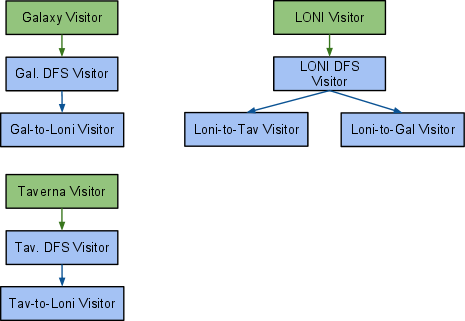
\includegraphics[width=\textwidth]{visitorinheritance.png}
\caption{Visitor inheritance tree.}
\label{fig:visitorinheritance}
\end{figure}

\paragraph{DFS Visitor}

Depth first search visitors visit all the nodes in a tree. They are useful for primarily diagnostic reasons.  By extending from the DFS visitor instead of implementing the interface, visit functions for each converter class can be written incrementally rather than implemented all at once. Un-overridden visit functions still visit the object thoroughly since they fall back to the DFS visitor. DFS visitors are also useful for troubleshooting OTS structure.

\paragraph{Interaction}

The Converter will interact with the main routine of the function. The OTS generated from the Parser will be passed into the visit function of the converter appropriate for the conversion request. All  the conversion will be done inside of the converter, and the desired tree will be recursively built. The built tree is then returned through the visit function. 

\subsection{Design Rationale}
The main justification behind the architectural design chosen was the separation of subsystems into entities that can stand on their own. The parser, converter, and generator have very specific duties that do not overlap with the other subsystems. The parser's input is a simple file and its output is an OTS. The converter's input is an OTS and its output is an OTS. The generator's input is an OTS and its output is a file. The symmetry, as depicted in figure~\ref{fig:architecture}, allows the entire system to be understood easily.  Since the components are not strongly coupled, separate parts of the program can be developed simultaneously with little integration cost.

Another factor that went into the decisions made were the libraries chosen for parsing and generating XML and JSON files. We found reflection-based parsers and generators to be the best for accommodating future changes to the file format's language. The functionality provided by the chosen libraries suggested a symmetrical system. Although this directed our design before we had a chance to consider many other alternatives, we believe the resulting architecture is sound.

The design was also created in a way so that it is extensible. All three major subsystems depend on rules that can be externalized and added to at a later point in time. If the creators of the workflow editors decide to add more modules or functionality, it will be possible for us or future developers to add and integrate the new functionality to the parser and generator fairly easily. Interfaces for the visitors were also written for the sake of extensibility. When adding a new feature for conversion, creating a new visit function in the interface forces the implementation of conversion functions wherever necessary.

The design for the converter is very flexible. Visitors provide a way of converting the entire tree by segmenting conversion tasks into small, node-level functions.  Visitors can be modified to accomplish a variety of complex tasks that may be required when converting very different file formats. for example, visitors can be modified to convert based on the context of the node through writing nested visitors. Specialized classes can be handled generically by omitting visit functions for the specialized class, or be handled specially by adding a visit function.  Visitors support complexities that should be anticipated when writing a converter.

\section{Data Description}



The overall flow of information in our program can be seen in figure~\ref{fig:dataflow}.

The information domain for our program are workflow files from LONI Pipeline (\texttt{.pipe} files), Taverna (\texttt{.t2flow} files), and Galaxy (\texttt{.ga} files). These are stored either on the local machine or on a server that the user has access to.  

In addition to the main formats, there are a few secondary data files used in the galaxy conversion case. Galaxy \texttt{.xml} tool specifications are stored separately from the \texttt{.ga} file in various sub-folders in the ``tools'' directory. These tools and their relative paths are listed in the \texttt{tool\_config.xml} file located in the root directory of the galaxy installation. The \texttt{tool\_config.xml} file is used by the program to generate a list of available tools. Using the path list parsed from the \texttt{tool\_config.xml} file, the tool .xml files used in the .ga file are loaded before conversion.

\begin{figure}
\centering
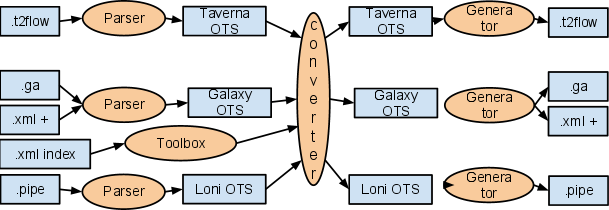
\includegraphics[width=\textwidth]{dataflow.png}
\caption{Data flow diagram.}
\label{fig:dataflow}
\end{figure}

Our program acts on one input data file (\texttt{.pipe}, \texttt{.t2flow}, or \texttt{.ga}) at a time (or several in the case of Galaxy). The first transformation on the input data takes the input file and creates the Object Tree Structure (OTS).

The OTS will be stored in main memory as instantiated objects. The example previously given in section~\ref{archdesign} illustrates the general structure of the classes that will be used to store the file data as an OTS. Elements, attributes, and content of XML files will be mapped to objects and fields of classes. The conversion process will simply change the OTS from one workflow representation to another. The output OTS will be stored similarly, but the names and layout of the classes will be different.

Once the output OTS has been created, the system will then turn that data into an output file via the generator. This file will be either a LONI Pipeline \texttt{.pipe} file, a Taverna \texttt{.t2flow} file, or a Galaxy \texttt{.ga} file. It will be created by the generator according to the binding rules given to it upon its creation by the specification. 

\section{Human Interface Design}

\subsection{Overview of User Interface}

The interface of the converter is a command-line interface. Users interact with the program on the command line of their system, using arguments passed to the program to specify the options they wish the program to use as well as the files to read from and write to. The command-line arguments should be parsed in a manner similar to that used by common UNIX utilities, so that no new knowledge of any particular syntax is needed.

Some command-line programs can later be extended with GUIs that simply call the program with arguments like a user would, but present to the user a graphical way to set options. The command-line interface should be compatible with such a GUI.

\begin{table}[htbp]
\begin{tabularx}{\textwidth}{| l | X |}
\hline
\texttt{-c}                                 & print output to stdout instead of to file (requires \texttt{--output-format}) \\
\hline
\texttt{-f,--force}                         & force (attempt to ignore errors) \\
\hline
\texttt{-g,--galaxy-app-dir <arg>}          & input directory for Galaxy \texttt{.xml} files \\
\hline
\texttt{-h,--help}                          & print this help \\
\hline
\texttt{-i,--input <arg>}                   & input file \\
\hline
\texttt{-j,--galaxy-output-app-dir <arg>}   & output directory for Galaxy \texttt{.xml} files \\
\hline
\texttt{-o,--output <arg>}                  & output file (if \texttt{-c} and \texttt{--output-format} not specified) \\
\hline
\texttt{-p,--output-format <arg>}           & output file format (if \texttt{--output} not specified or if \texttt{-c} specified) \\
\hline
\texttt{-v,--verbose}                       & be verbose (print debug messages to stderr) \\
\hline
\end{tabularx}
\caption{A summary of valid command line arguments.}
\label{argstable}
\end{table}

The user must at least provide one input file (\texttt{-i}) and some type of output argument (\texttt{-o}, \texttt{-p}) to run the converter successfully. Other valid command line arguments are specified in table~\ref{argstable}.

The program will print error messages if the command-line arguments are insufficient or contain errors. The program will also print messages if there are any errors in the conversion. Since the standard output stream is a valid destination for the conversion, error messages and other information will be printed to standard error.

\subsection{Screen Image}

As seen in the command-line interface demo in figure~\ref{fig:screenshot}, the program prints a very helpful message describing the options available. It supports a ``verbose'' option, where it prints more information about what it's doing. It also properly errors out when invalid input is given. 

\begin{figure}[htbp]
\centering
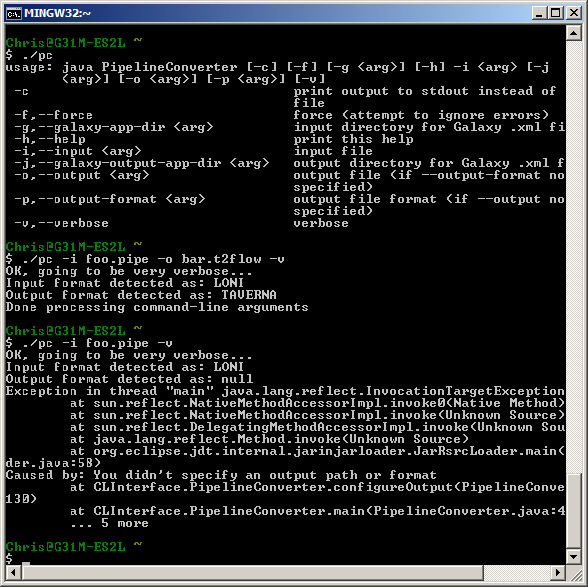
\includegraphics[width=0.90\textwidth]{screenshot.png}
\caption{Screenshot of the program.}
\label{fig:screenshot}
\end{figure}
\end{document}
